\chapter{Terminologies}

\begin{itemize}
	\item Le client est le commanditaire du projet.
	\item Un utilisateur est une personne souhaitant utiliser un logiciel du client. 
	\item Une licence est un droit accordé pour une machine et un utilisateur d'utiliser un logiciel donné.
	\item Craquer un logiciel est le fait de pouvoir l'utiliser sans avoir payé pour son utilisation. Soit en modifiant le code compilé, soit en utilisant une autre méthode. 
\end{itemize}

\chapter{Contexte du projet}

Ce projet s’intitulant “Gestion et protection de licence” est proposé par notre client \\Mr.
Ziadi.\\\newline Il a pour but de créer une ou plusieur application de gestion, génération et protection 
de licence, plus particuliairement un gestionnaire de licence pour les logiciels créés par monsieur Ziadi.
\\ \newline Dans notre cas ce projet a pour but de nous apporter des connaissances et de l'experience dans les domaines traités
 mais aussi de valider notre 1 ère année de Master Informatique en Sécurité des Systèmes d’Information (SSI).\\ \newline
Nous pouvons être amenés à travailler avec Mr. Macadré pour tout ce qui est
serveur et gestion de machine virtuelles (pour leurs mise en place).\\ Nous
nous appuyons sur la Spécification Technique de Besoin, le Document d'Architecture
Logicielle, le Cahier de Recette, l’Analyse des Risques, et sur ce Plan de Développement
pour conduire le projet.

\chapter{Méthodologie de développement}

Depuis le début du projet nous travaillons selon un fonctionnement agile, avec des
réunions et des livrables réguliers, avec le client. Ce fonctionnement permet de produire de
la valeur rapidement.\\ \newline
Nous avons choisi de commencer le développement de l’application par les vues car
nous sommes partis du principe que le but final de ce projet était de rendre une application,
avec des rendus tout au long du semestre. Commencer par les vues nous permettra d’avoir
un visuel le plus rapidement possible, et d’obtenir un prototype manipulable, pour l’ensemble
des livrables.\\ \newline
Ces prototypes ne contiendront bien sûr pas l’ensemble des fonctionnalités finales
attendues par le client, mais nous permettront de réagir plus rapidement sur l’ajout de
fonctionnalités dans l’application, en fonction des demandes de ce dernier, mais nous
permettra également de faire les tests des attaques plus simplement en nous assurant que
les vues sont correctement implémentées.\\ \newline
Après avoir implémenter les vues qui permettent de naviguer entre elles, nous
commencerons par implémenter le modèle de protection et de gestion des licences.\\ \newline

La sécurité etant au coeur de notre projet, les element tel que l'obfuscation, l'injection de code et la partie 
gestion et securisation de base de données seront des element pouvouvant être gérés en divisant nos ressources
car ils sont facilement implémentable aux projet final.

\chapter{Organisation et responsabilités}

Pour organiser ce projet et travailler efficacement, nous avons affecté un rôle à
chacun. Néanmoins, tous les acteurs de ce projet auront les rôles de développeur et de
rédacteur. Voici notre organigramme :\\ \newline


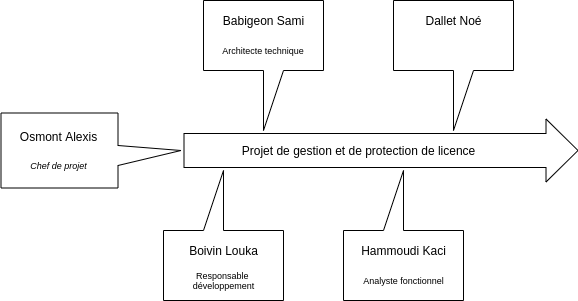
\includegraphics[width=15cm]{schema_role_projet.png}
\\ \newline
\begin{itemize}
	\item  \textbf{Chef de projet :} \newline
	\begin{itemize}
		\item Organiser et conduire le projet de bout en bout.
		\item Décide des actions et résout les désaccords entre les membres du projet.\newline
	\end{itemize}
	\item \textbf{Architecte tehcnique :} \newline
	\begin{itemize}
		\item Garantit l'encadrement et la maintenance technique du projet.
		\item Assure la fiabilité, la performance et l'évolution du système d'information.\newline
	\end{itemize}
	\newpage
	\item \textbf{Analyste fonctionnel :} \newline
	\begin{itemize}
		\item Schématise l’interface de l’application.
		\item Se charge de la conception générale de l’interface, de la clarté de la
		navigation, de l’optimisation des parcours ainsi que de la qualité des
		contenus.\newline
	\end{itemize}
	
	\item \textbf{Responsable développement :} \newline
	\begin{itemize}
		\item Définit les besoins du client.
		\item Assure le suivi fonctionnel.\newline
	\end{itemize}
	
	
\end{itemize}

\chapter{Organigramme des tâches}
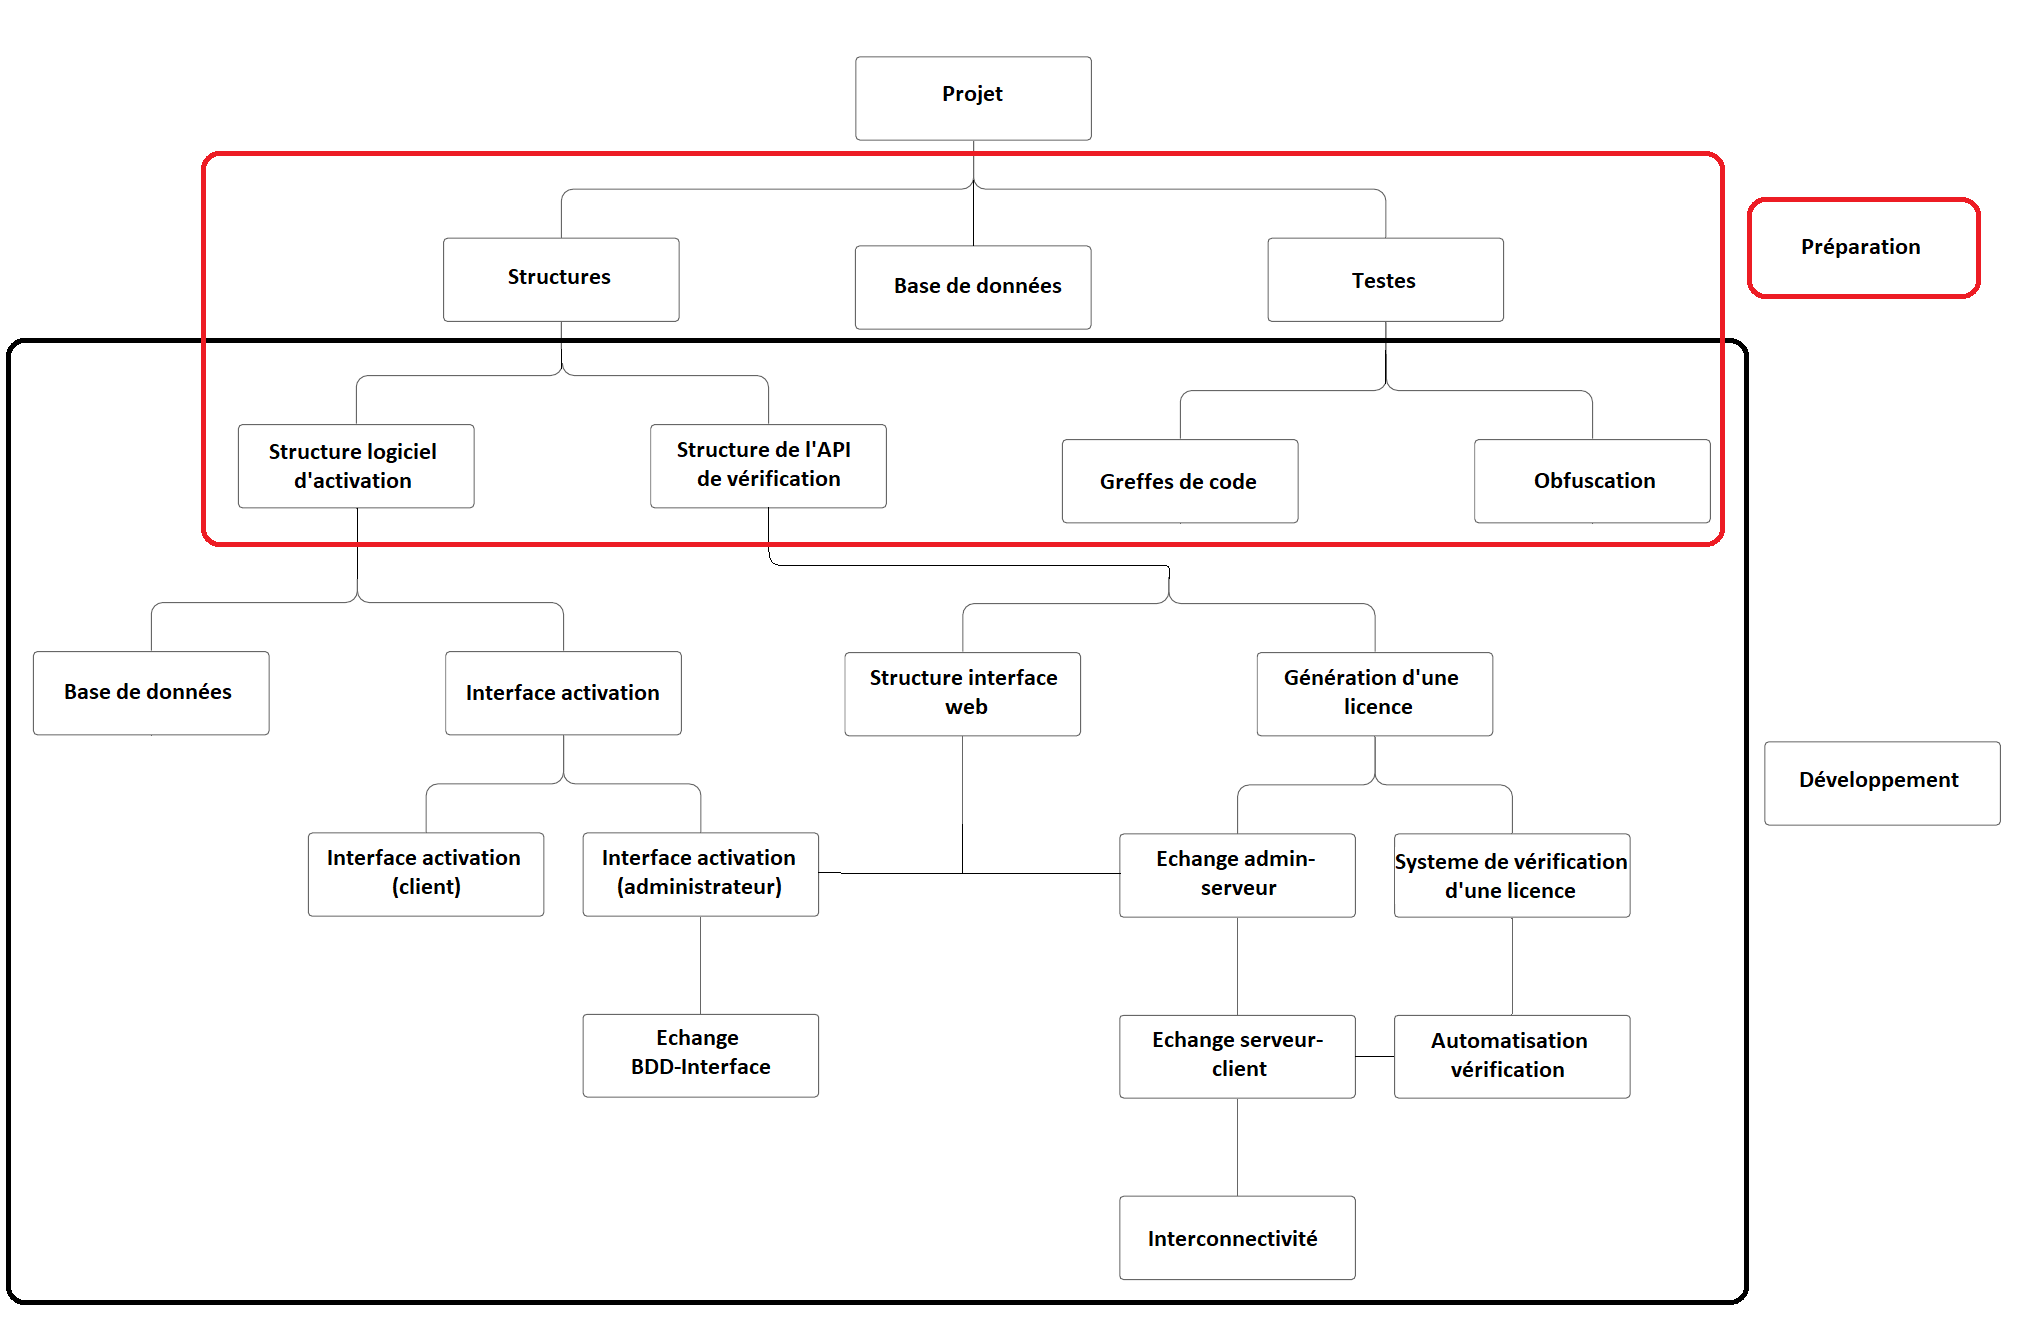
\includegraphics[width=15cm]{organi2png.png}

\chapter{Evaluation du projet et dimensionnement des moyens}
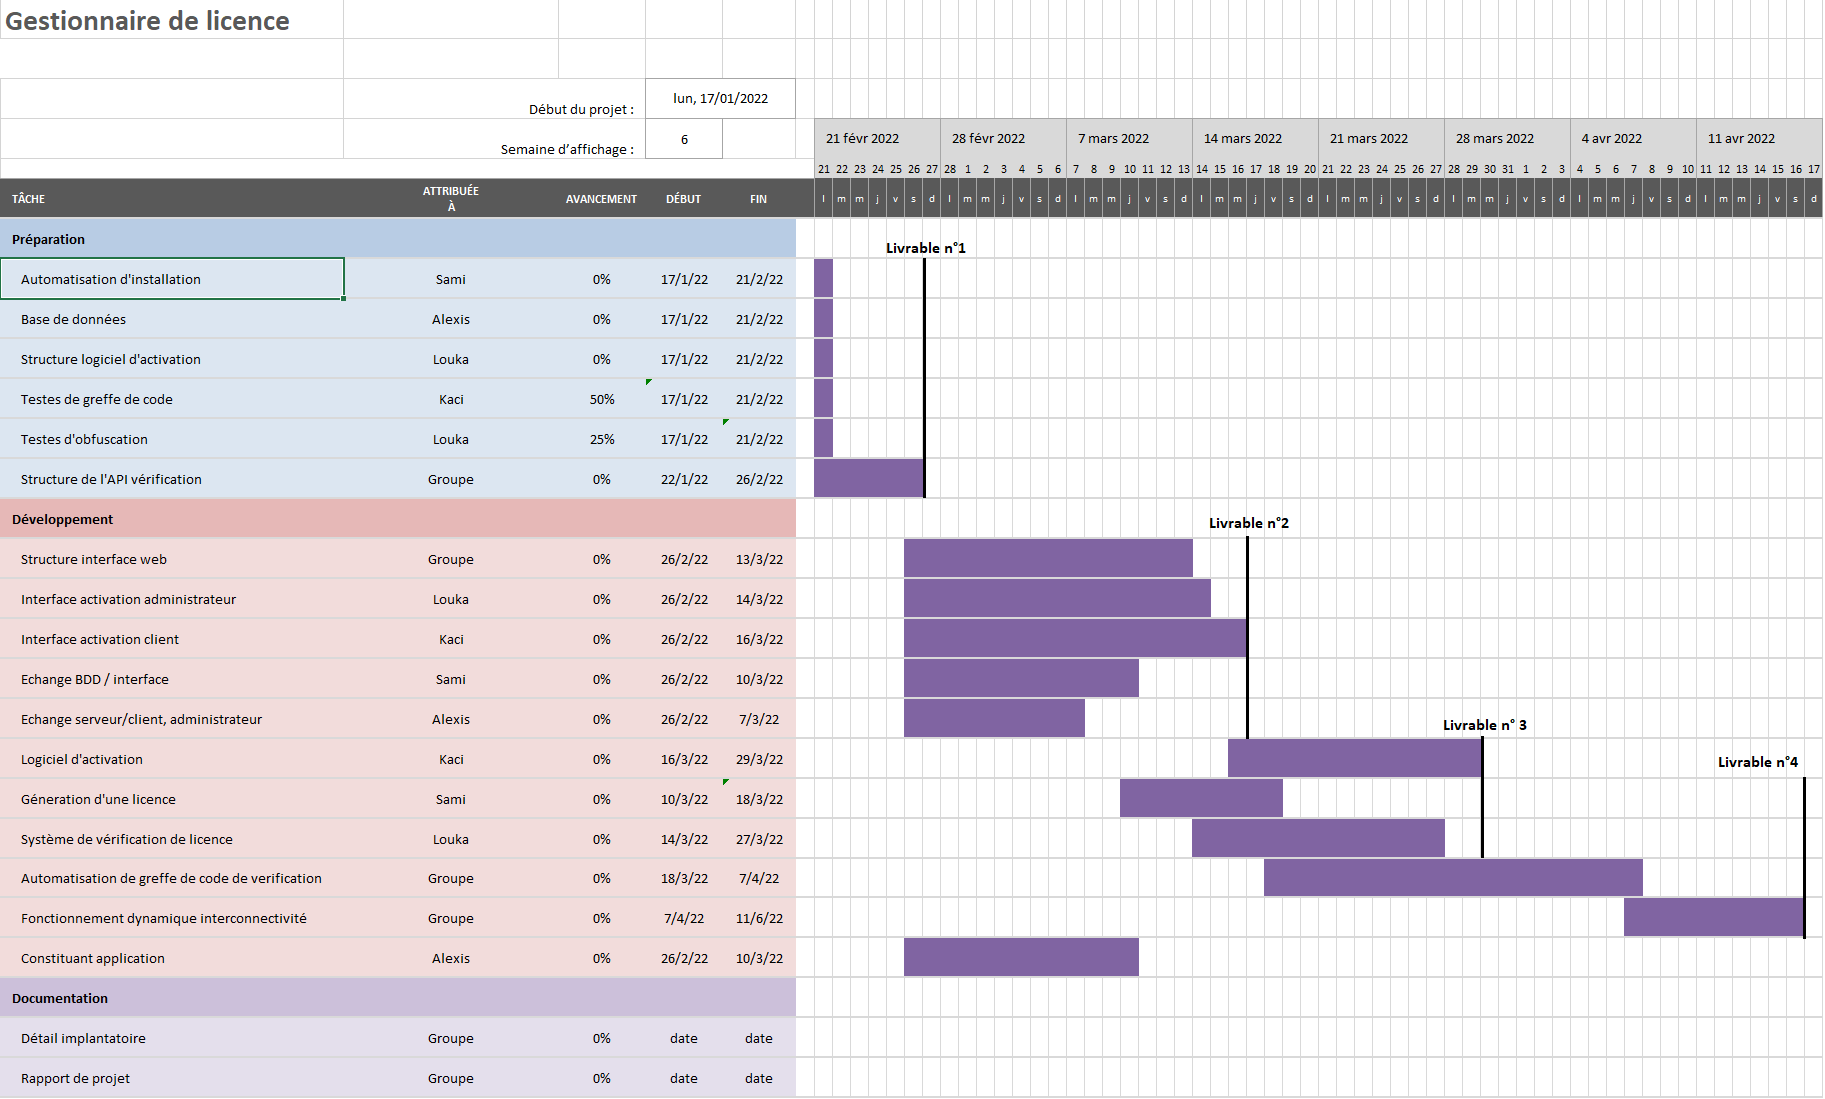
\includegraphics[width=15cm]{Gantt.png}

\chapter{Planning général}

\chapter{Procédés de gestion}
\subsection{Gestion de la documentation}
		Au second semestre, nous devrons fournir les documents suivants :
		\begin{itemize}
			\item Documentation technique : décrit le fonctionnement détaillé de l’application.
			\item Notice d’utilisation : support explicatif du maniement de l’application.
			\item Étude du domaine : état de l’art du domaine, des contre-mesures et des
			réglementations de vigueur.
			\item Des livrables pré-réunion chaque deux semaine.\\ \newline
		\end{itemize}
	
		\subsection{Gestion des configurations}
		Lors du développement, nous utiliserons le GitLab fourni par l’université ainsi que github. Chacun
		aura une tache de développement et il y aura des réunion de travail en groupe qui donneront les versions
		stable du code (pré-réunion) et des documentations (en Latex). Chacun aura son espace pour
		permettre a tous de fusionner sa partie à la branche principale.



\chapter{Revues et points clefs}

L'objectif dans notre cas est de faire suivre notre projet par note client,
nous fournirons donc au client un livrable toutes les deux semaines, et nous effectuerons
quelques jours après chaque livraison une réunion avec lui pour voir les modifications à
apportées. Des dates prévisionnelles ont été indiquées dans le diagramme de Gantt.

\chapter{Procédure de suivi d'avancement}

Pour avancer rapidement et efficacement tout en évitant les hors-sujet, nous avons
décidé d’utiliser diverses plateformes pour suivre l’avancement de chacun, et de ce fait,
d’éviter qu’un membre ne soit en attente. Les plateformes utilisées sont les suivantes :\\ \newline

\begin{itemize}
	\item Discord :\\
	Cet outil nous permet de communiquer rapidement entre nous et
de faire des audios / visioconférences pour nos réunions. Il est aussi très utile
pour communiquer rapidement et faire des annonces importantes (réunions,
vérification d’un mail avant son envoi, etc.) et pour partager / archiver les
comptes rendus de toutes les réunions.\\
	\item Trello :\\
	Cet outil nous permet de répartir et de savoir sur quelle tâche
travaillent les membres de l’équipe et de connaître leur avancement.\\
	\item GitHub :\\
	L’université nous a fourni cet outil qui est très pratique pour stocker
les documentations produites et le code source de l’application que nous
aurons à faire lors de la phase de développement.\\
	\item Google docs / GitHub :\\
	Ces outils nous permettent de réaliser les documents demandés
pour la matière Gestion de Projet. Google Docs nous permet de travailler à
plusieurs sur un même document. Les modifications apparaissent en temps
réel et sont sauvegardées sur une période de trente jours. Il est donc possible
de consulter des versions antérieures de nos documents en quelques clics.\\
	\item Réunions :\\
	Le meilleur moyen de travailler efficacement reste le fait d'organiser des réunions en physique 
	plutot que des appels ou des echanges de messages. C'est pourquoi nous organisons régulièrement des réunions
	entre membre du projet pour faire un point définir les objectif et avancer sur le projet.
\\ \newline

Pour tenir de l'avancement du projet nous planifions des seances de travails et des réunions hebdomadaire pour traiter
aussi bien de l'aspect technique que de l'aspect gestion de projet.
\end{itemize}
